\documentclass{article}

\usepackage{tikz}

\usetikzlibrary{positioning}

\begin{document}


\begin{figure}
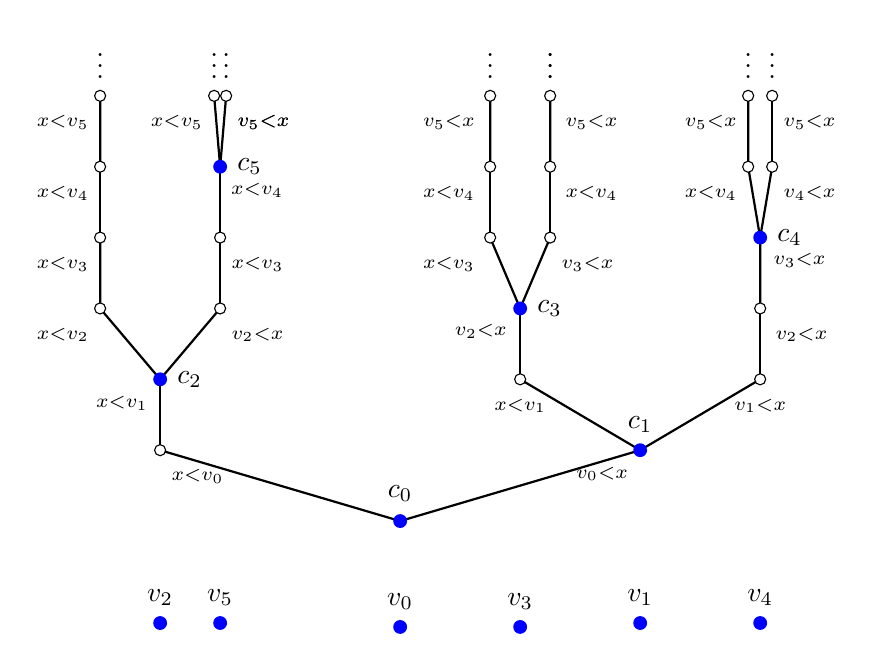
\begin{tikzpicture}[grow'=up,scale=.6]
\tikzstyle{level 1}=[sibling distance=4in]
\tikzstyle{level 2}=[sibling distance=2in]
\tikzstyle{level 3}=[sibling distance=1in]
\tikzstyle{level 4}=[sibling distance=0.5in]
\tikzstyle{level 5}=[sibling distance=0.2in]
\tikzstyle{level 6}=[sibling distance=0.1in]
\tikzstyle{level 7}=[sibling distance=0.07in]
\node [label=$c_0$] {} coordinate (t9)
child{ coordinate (t0) edge from parent[color=black,thick]
child{ coordinate (t00) edge from parent[color=black,thick]
%edge from parent node[right] {help}
child{ coordinate (t000) edge from parent[color=black,thick]
child{coordinate (t0000) edge from parent[color=black,thick]
child{coordinate (t00000) edge from parent[color=black,thick]
child{coordinate (t000000) edge from parent[color=black,thick]}
}%endparen for t00000
}%endparen for t0000
}%endparen for t000
child{ coordinate (t001) edge from parent[color=black,thick]
child{ coordinate (t0010) edge from parent[color=black,thick]
child{coordinate (t00100) edge from parent[color=black,thick]
child{coordinate (t001000) edge from parent[color=black,thick]}
child{coordinate (t001001) edge from parent[color=black,thick]}
}%endparen for t00100
}%endparen for t0010
}%closeparen for t001
}%endparen for t00
%child{coordinate (t01) edge from parent[color=white]} 
}%endparen for t0
child{ coordinate (t1) edge from parent[color=black,thick]
child{ coordinate (t10) edge from parent[color=black,thick]
child{ coordinate (t100)
child{coordinate (t1000)
child{coordinate (t10000)
child{coordinate (t100000)}
}%endparen for t10000
}%endparen for t1000
child{coordinate (t1001)
child{coordinate (t10010)
child{coordinate (t100100)}
}%endparen for t10010
}%endparen for t1001
}%endparen for t100
}%endparen for t10
child{ coordinate (t11) [label={\small 1/16}]
child{coordinate (t110)
child{coordinate (t1100)
child{coordinate (t11000)
child{coordinate (t110000)}
}%endparen t11000
child{coordinate (t11001)
child{coordinate (t110010)}
}%endparen for t11001
}%endparen for t1100
}%endparen for t110
}%endparen for t11
}%endparen for t1
;
%line spaces make a difference!!!


\node[circle, fill=blue,inner sep=0pt, minimum size=5pt] at (t9) {};
\node[circle, fill=blue,inner sep=0pt, minimum size=5pt,label=0:$c_2$,label=250:$\scriptstyle{x<v_1}$] at (t00) {};
\node[circle, fill=blue,inner sep=0pt, minimum size=5pt,label=0:$c_5$,label=280:${\scriptstyle x<v_4}$] at (t00100) {};
\node[circle, fill=blue,inner sep=0pt, minimum size=5pt, label=$c_1$,label=250:$\scriptstyle{v_0<x}$] at (t1) {};
\node[circle, fill=blue,inner sep=0pt, minimum size=5pt, label = 0:$c_3$,label=240:$\scriptstyle{v_2<x}$] at (t100) {};
\node[circle, fill=blue,inner sep=0pt, minimum size=5pt,label = 0:$c_4$,label=300:$\scriptstyle{v_3<x}$] at (t1100) {};
\node[label=280:$\scriptstyle{x<v_0}$] at (t0) {};
\node[label=270:$\scriptstyle{v_1 < x}$] at (t11) {};
\node[label=270:$\scriptstyle{x<v_1}$] at (t10) {};
\node[label=300:$\scriptstyle{v_2 < x}$] at (t110) {};
\node[label=240:${\scriptstyle x<v_3}$] at (t1000) {};
\node[label=280:${\scriptstyle v_3 < x}$] at (t1001) {};
\node[label=240:${\scriptstyle x<v_4}$] at (t10000) {};
\node[label=300:${\scriptstyle x < v_4}$] at (t10010) {};
\node[label=240:${\scriptstyle v_5<x}$] at (t100000) {};
\node[label=300:${\scriptstyle v_5<x}$] at (t100100) {};
\node[label=260:${\scriptstyle x<v_4}$] at (t11000) {};
\node[label=280:${\scriptstyle v_4<x}$] at (t11001) {};
\node[label=260:${\scriptstyle v_5<x}$] at (t110000) {};
\node[label=280:${\scriptstyle v_5<x}$] at (t110010) {};
\node[label=260:${\scriptstyle x<v_2}$] at (t000) {};
\node[label=280:${\scriptstyle v_2<x}$] at (t001) {};
\node[label=260:${\scriptstyle x<v_3}$] at (t0000) {};
\node[label=280:${\scriptstyle x<v_3}$] at (t0010) {};
\node[label=260:${\scriptstyle x<v_4}$] at (t00000) {};
\node[label=260:${\scriptstyle x<v_5}$] at (t000000) {};
\node[label=260:${\scriptstyle x<v_5}$] at (t001000) {};
\node[label=280:${\scriptstyle v_5<x}$] at (t001001) {};
\node[label=280:${\scriptstyle v_5<x}$] at (t001001) {};

%the dots going up
\node[circle,inner sep=0pt, minimum size=5pt,label=90:$\vdots$] at (t000000) {};
\node[circle,inner sep=0pt, minimum size=5pt,label=90:$\vdots$] at (t001000) {};
\node[circle,inner sep=0pt, minimum size=5pt,label=90:$\vdots$] at (t001001) {};
\node[circle,inner sep=0pt, minimum size=5pt,label=90:$\vdots$] at (t100000) {};
\node[circle,inner sep=0pt, minimum size=5pt,label=90:$\vdots$] at (t100100) {};
\node[circle,inner sep=0pt, minimum size=5pt,label=90:$\vdots$] at (t100100) {};
\node[circle,inner sep=0pt, minimum size=5pt,label=90:$\vdots$] at (t110000) {};
\node[circle,inner sep=0pt, minimum size=5pt,label=90:$\vdots$] at (t110010) {};%#current 

%empty circle nodes
\node[circle, fill=white,draw,inner sep=0pt, minimum size=4pt] at (t0) {};
\node[circle, fill=white,draw,inner sep=0pt, minimum size=4pt] at (t000) {};
\node[circle, fill=white,draw,inner sep=0pt, minimum size=4pt] at (t0000) {};
\node[circle, fill=white,draw,inner sep=0pt, minimum size=4pt] at (t00000) {};
\node[circle, fill=white,draw,inner sep=0pt, minimum size=4pt] at (t000000) {};
\node[circle, fill=white,draw,inner sep=0pt, minimum size=4pt] at (t001) {};
\node[circle, fill=white,draw,inner sep=0pt, minimum size=4pt] at (t0010) {};
\node[circle, fill=white,draw,inner sep=0pt, minimum size=4pt] at (t001000) {};
\node[circle, fill=white,draw,inner sep=0pt, minimum size=4pt] at (t001001) {};
\node[circle, fill=white,draw,inner sep=0pt, minimum size=4pt] at (t10) {};
\node[circle, fill=white,draw,inner sep=0pt, minimum size=4pt] at (t1000) {};
\node[circle, fill=white,draw,inner sep=0pt, minimum size=4pt] at (t10000) {};
\node[circle, fill=white,draw,inner sep=0pt, minimum size=4pt] at (t100000) {};
\node[circle, fill=white,draw,inner sep=0pt, minimum size=4pt] at (t1001) {};
\node[circle, fill=white,draw,inner sep=0pt, minimum size=4pt] at (t10010) {};
\node[circle, fill=white,draw,inner sep=0pt, minimum size=4pt] at (t100100) {};
\node[circle, fill=white,draw,inner sep=0pt, minimum size=4pt] at (t11) {};
\node[circle, fill=white,draw,inner sep=0pt, minimum size=4pt] at (t110) {};
\node[circle, fill=white,draw,inner sep=0pt, minimum size=4pt] at (t11000) {};
\node[circle, fill=white,draw,inner sep=0pt, minimum size=4pt] at (t110000) {};
\node[circle, fill=white,draw,inner sep=0pt, minimum size=4pt] at (t11001) {};
\node[circle, fill=white,draw,inner sep=0pt, minimum size=4pt] at (t110010) {};

%the nodes along the bottom
\node[circle, fill=blue,inner sep=0pt, minimum size=5pt, label=$v_2$,below=3cm of t00] (v2) {};
\node[circle, fill=blue,inner sep=0pt, minimum size=5pt,label=$v_5$,below =3.9cm of t001] (v5) {};
\node[circle, fill=blue,inner sep=0pt, minimum size=5pt,label=$v_0$,below =1.25cm of t9] (v0) {};
\node[circle, fill=blue,inner sep=0pt, minimum size=5pt,label=$v_3$,below =3.95cm of t100] (v3) {};
\node[circle, fill=blue,inner sep=0pt, minimum size=5pt,label=$v_1$,below =2.1cm of t1] (v1) {};
\node[circle, fill=blue,inner sep=0pt, minimum size=5pt,label=$v_4$,below =3cm of t11] (v4) {};
\end{tikzpicture}
\end{figure}


\end{document}